\documentclass[12pt]{article}

\usepackage{mathtools}
\usepackage{geometry}
\usepackage{graphicx}
\usepackage[hidelinks]{hyperref}
\usepackage{bm}
\usepackage{amssymb}
\usepackage{dsfont}
\usepackage[most]{tcolorbox}

\geometry{a4paper,
textwidth=18cm,
top=1.5cm,
bottom=1.5cm}

\newcommand{\minisection}[1]{
    \par\vspace{0.25cm}
    \textbf{#1}\par
    \vspace{0.1cm}
    \hrule
    \vspace{0.25cm}
}

\newcommand{\doubleline}{
    \hrule
    \vspace*{0.05cm}
    \hrule
    \vspace*{0.25cm}
}

\DeclareMathOperator{\var}{var}
\DeclareMathOperator{\cov}{cov}
\DeclareMathOperator{\cor}{cor}

\newcommand{\idop}{\hat{\mathds{1}}}

\setlength\parindent{0pt} 

\begin{document}
    \doubleline
    \begin{center}
        \huge \textbf{Stats Notes}
    \end{center}
    \doubleline
    % --------
    \minisection{Maximum Likelihood}
    Say that we take samples from a probability density function $f(x;\theta)$, where $x$ is an observed value, and $\theta$ some parameter. One problem to consider would be estimating $\theta$ given a set of measurements ${x_i}$ - to do this, we can define the \textit{likelihood} as:
    \begin{equation*}
        L(\theta) = f(\bm x;\theta)
    \end{equation*}
    For random samples (drawn from the same distribution), this is simply:
    \begin{equation*}
        L(\theta) = \prod_{i}f(x_i;\theta)
    \end{equation*}
    If the samples are drawn from different distributions, then:
    \begin{equation*}
        L(\theta) = \prod f_i(x_i;\theta)
    \end{equation*}
    $\theta$ might be a vector of parameters - if we \textbf{minimise} the likelihood with respect to these parameters, then we can find a \textit{maximum likelihood estimate}, $\hat\theta(\bm x)$.\\
    We can also find the same result by maximising the \textit{log-likelihood}, i.e. $\ell(\theta)=\ln L(\theta)$. This may be more convenient.
    % --------
    \minisection{Estimators}
    Any function of observations $X_i$, $T(X_i)$, may act as an \textit{estimator} for some parameter (e.g. the maximum likelihood). The mean-squared error of an estimator is:
    \begin{equation*}
        \text{MSE}(T) = E[(T-\theta)^2]
    \end{equation*}
    Here, $E[\cdot]$ signifies an expectation value. Furthermore, the bias is given:
    \begin{equation*}
        b(T) = E(T) - \theta
    \end{equation*}
    In both cases, $\theta$ is the parameter which the estimator estimates. An unbiased estimator has $b=0$.
    % --------
    \minisection{Regression}
    We can model a linear fit for a dataset $y_i$ as being drawn from a set of random variables, $Y_i$:
    \begin{equation*}
        Y_i = \alpha + \beta x_i + \epsilon_i
    \end{equation*}
    Here, $x_i$ are known constants, $\alpha,\beta$ unknown paramters, and $\epsilon_i$ a set of `random errors'. In fact, this is a normal distribution, with $Y_i\sim N(\alpha+\beta x_i,\sigma^2)$, and we can assume that $\sigma^2$ is known. Then, the log-likelihood is:
    \begin{equation*}
        \ell(\alpha,\beta) = -\frac n2\ln(2\pi\sigma^2) - \frac{1}{2\sigma^2}\sum_i\big( y_i-\alpha-\beta x_i\big)^2
    \end{equation*}
    The first term is just a constant, so we find that \textit{maximising} the likelihood is \textbf{equivalent} to \textit{minimising} the sum of squares:
    \begin{equation*}
        S(\alpha,\beta) = \sum_i\big( y_i - \alpha - \beta x_i \big)^2
    \end{equation*}
    As such, the MLEs of $\alpha$ and $\beta$ are known as the \textit{least-squares estimators}.\\
    In the general case, a linear model depends on any number of explanatory variables, $x^{(i)}_j$:
    \begin{equation*}
        Y_j = \beta_0 + \sum_{i=1} \beta_ix_j^{(i)}
    \end{equation*}
    Then, the least-squares estimates are given by minimising:
    \begin{equation*}
        S(\bm\beta) = \sum_{j}\left( y_j - \beta_0 + \sum_{i=1}\beta_i x_j^{(i)}\right)
    \end{equation*}
    We have thus far assumed that $\sigma^2$ is the same for all measurements, but if this is not the case, then we can perform a \textit{weighted} least-squares minimisation:
    \begin{equation*}
        \sum_i w_i\big(y_i - \alpha - \beta x_i\big)^2
    \end{equation*}
    Here, $w_i\propto \sigma_i^{-2}$, so points with smaller uncertainty will be reflected more. 
    % ---------
    \minisection{Joint Probability Distribution}
    If we are working with multiple random variables (e.g. $x,y$), then we can represent their measurements as a \textit{joint} probability distribution, $f(x,y)$. This may include some correlation between the two, i.e. loss of symmetry.\\
    We can recover the \textit{marginal} distributions, which describe the probability of a single measurement, by integrating the joint distribution over the other measurement:
    \begin{align*}
        f_X(x) = \int f(x,y)\ \text dy && f_Y(y) = \int f(x,y)\ \text dx
    \end{align*}
    % ---------
    \minisection{Multivariate Normal Distribution}
    The multivariate normal distribution is a generalisation of the univariate normal distribution to arbitrary higher dimensions, i.e. a $p$-dimensional column vector $X=(X_1,\cdots,X_p)^T$. It allows for nonzero correlations to exist between vector elements (important!).\\
    For said $p$-dimensional random column vector, $X$, we say that $X$ has a multivariate normal distribution, with a vector of means $\mu = (\mu_1,\cdots,\mu_p)^T$, and a $p\times p$ \textit{covariance} matrix, $\Sigma$, so that the \textit{joint} pdf of $X$ is:
    \begin{equation*}
        f(x) = \frac{1}{(2\pi)^{\frac p2}\left|\Sigma\right|^{\frac 12}}\exp\left(-\frac 12\big( x-\mu\big)^T\Sigma^{-1}\big( x-\mu\big)\right)
    \end{equation*}
    Here, $x\in \mathbb R^p$, i.e. a real column vector.\\
    This covariance matrix, $\Sigma$, is key! If the measurements were all independent, then the off diagonal terms would clearly be zero, but by choosing them to be nonzero, we allow for a level of correlation between the different dimensions (this will be important). Specifically, we can interpret:
    \begin{align*}
        \mathbb E[X_i] &= \mu_i & \var(X_i) &= \Sigma_{ii} & \cov(X_i,X_j) &= \Sigma_{ij}\\
        & & & & &\hphantom{=}(i\neq j)
    \end{align*}
    $\text{cov}\ (X_i,X_j)$, the covariance of two dimensions $X_i$ and $X_j$, is a measure of their respective (linear) correlation, i.e. the tendency in their mutual linear relationship. A value of zero would (likely) indicate that they were independent (or non-linearly correlated). If the covariance is equal to the variance, it would indicate that the variables were \textit{identical}.\\
    Formally, we can define the \textit{correlation} between these variables as:
    \begin{equation*}
        \cor(X_i,X_j) \equiv \frac{\cov(X_i,X_j)}{\sqrt{\var(X_i)\var(X_j)}} = \frac{\Sigma_{ij}}{\sqrt{\Sigma_{ii}\Sigma_{jj}}}
    \end{equation*}
    % --------
    \minisection{Simulating a Multivariate Distribution}
    An important process to understand is that of drawing samples from a multivariate normal distribution - evidently, this will be somewhat complicated, given that we have to account for correlation between dimensions.\\
    Here, I will outline a common method for achieving this:
    \begin{enumerate}
        \item Given the covariant matrix, $\Sigma$, we must find a matrix $A$ which satisfies:
        \begin{equation*}
            AA^T = \Sigma
        \end{equation*}
        If $\Sigma$ is positive-definite, we can use the \textit{Cholesky decomposition}, i.e. $\text{chol}(\Sigma) = A^T$. We may also use a \textit{SVD decomposition}. 
        \item Next, we want to generate a vector of independent standard normal variables, i.e. $\bm z\in \mathbb R^n$, where $z\sim N(0,1)$.
        \item Finally, our random vector is given by:
        \begin{equation*}
            \bm x = \bm\mu+A\bm z
        \end{equation*}
    \end{enumerate}
    Given a set of observations from a multivariate normal distribution, we can make parameter estimations as
    \begin{equation*}
        \hat\mu = \frac 1n\sum_ix_i
    \end{equation*}
    for the mean, and
    \begin{equation*}
        \hat\Sigma = \frac 1n\sum_i (x_i - \hat\mu)(x_i - \hat\mu)^T.
    \end{equation*}
    Keep in mind that $x_i$ and $\hat\mu$ are \textit{vector} quantities. The above for $\hat\Sigma$ is biased; an unbiased estimator is:
    \begin{equation*}
        \bm S = \frac{1}{n-1}\sum_i(x_i-\hat\mu)(x_i-\hat\mu)^T
    \end{equation*}
    This is the sample covariance matrix. We may also find it useful to calculate the sample correlation matrix:
    \begin{equation*}
        \bm R_{ij} = \frac{\bm S_{ij}}{\sqrt{\bm S_{ii}\bm S_{jj}}}
    \end{equation*}
    % --------
    \minisection{Bayesian Inference}
    Say that we have a joint pdf, $f(y,z)$ - then the distributions of $y,z$ \textit{given} a fixed value of $z,y$ are, respectively:
    \begin{align*}
        f(z\ |\ y) = \frac{f(y,z)}{f(y)} && f(y\ |\ z) = \frac{f(y,z)}{f(z)}
    \end{align*}
    Substituting one into the other, we have Bayes' theorem (for continuous random variables):
    \begin{equation*}
        f(z\ |\ y) = \frac{f(y\ |\ z)f_Z(z)}{f_Y(y)}
    \end{equation*}
    The respective marginal densities are given by integrating as before.\\
    Now, say that we have some unknown parameter $\theta$ - we have a probability model for data $\bm x$, $f(\bm x\ |\ \theta)$, which is conditional on the value of $\theta$. Suppose that, before observing $\bm x$, we summarise our expectations (beliefs) about $\theta$ in a \textit{prior} density, $\pi(\theta)$. Since $\bm x$ is observed (i.e. fixed), $f(\bm x)$ is a constant.\\
    Via Bayes' theorem, we can then \textit{infer} a \textit{posterior} density, $f( \theta\ |\ \bm x)$, i.e. our updates beliefs about $\theta$, given our obversations of $\bm x$:
    \begin{equation*}
        \pi(\theta\ |\ \bm x) = \frac{f(\bm x\ |\ \theta)\cdot\pi(\theta)}{f(\bm x)} \propto f(\bm x\ |\ \theta)\cdot\pi(\theta)
    \end{equation*}
    We can then find the constant of proportionality through normalising the posterior density.\\
    Useful quantities can be drawn from the posterior density, e.g. mode, mean, median, variance, etc. These help us to classify our beliefs about the value of $\theta$.\\
    The Bayesian equivalent of a confidence interval is a \textit{credible} (or \textit{posterior}) interval. Specifically, a $100(1-\alpha)\%$ credible set for $\theta$ is a subset $C$ of $\Theta$, such that:
    \begin{equation*}
        \int_C \pi(\theta\ |\ \bm x)\ \text d\theta = 1-\alpha
    \end{equation*}
    That is, $P(\theta\in C\ |\ \bm x)=1-\alpha$.\\
    In the case of multiple parameters, the same techniques apply, but we must interpret the posterior density as a \textit{joint} density. As such, to find the marginal posterior of a single parameter (e.g. $\psi$), we integrate over all over components of $\pi(\psi,\lambda,\cdots)$.
    % --------
    \minisection{Prediction}
    Now, let $X_{n+1}$ be some future observation, and $\bm x$ our previously observed data. We will assume that, conditional on $\theta$, $X_{n+1}$ has density $f(x_{n+1}\ |\ \theta)$, independent of $X_1,X_2,\cdots,X_n$.\\
    The density of $X_{n+1}$ given $\bm x$, $f(x_{n+1}\ |\ \bm x)$, is known as the \textit{posterior predictive density}. We can express this as:
    \begin{align*}
        f(x_{n+1}\ |\ \bm x) &= \int f(x_{n+1},\theta\ |\ \bm x)\ \text d\theta\\
        &= \int f(x_{n+1}\ | \theta,\bm x)\pi(\theta\ |\ \bm x)\ \text d\theta
    \end{align*}
    The final line results from the identity that $f(u,v|w) = f(u|v,w)f(v|w)$.\\
    Due to independence, though, we can write that $f(x_{n+1}\ |\ \theta,\bm x) = f(x_{n+1}\ |\ \theta)$. Then:
    \begin{equation*}
        f(x_{n+1}\ |\ \bm x) = \int f(x_{n+1}\ |\ \theta)\pi(\theta\ |\ \bm x)\ \text d\theta
    \end{equation*}
    As such, given $\bm x$, the predictive density is found from combining the density for $x_{n+1}$ under the model (i.e. $f(x_{n+1}\ |\ \theta)$) with the posterior density.
    % --------
    \minisection{Choosing a Prior}
    One potential source of ambiguity is in the choosing of the prior - this represents our beliefs about the parameters `prior' to collecting data. We might:
    \begin{enumerate}
        \item Use the `guess' of an expert - say that a scientific expert anticipates a parameter $\theta$ to be around $10$, e.g. $\theta\in(5,17)$ with a probability of $0.95$.\\
        We might ask several different experts for their beliefs, and repeat analysis with this set of priors.
        \item If we have little prior knowledge, we might seek a form expressing `prior ignorance'. For example, if we were unsure of a probability, we might consider a uniform prior, e.g. $\theta\sim U(0,1)$ (though this may lead to problems when there are a large number of parameters).
    \end{enumerate}
    A prior, $\pi(\theta)$, is called `proper' if $\int \pi(\theta)\ \text d\theta = 1$, and improper if the integral can not be normalised (e.g. divergent). Improper priors can lead to a proper posterior, which may be used for inference. However, improper posteriors can \textbf{not} be used for inference.\\
    A particular choice of prior is a \textit{Jeffreys prior}, which has form
    \begin{equation*}
        \pi(\theta) \propto i(\theta)^{\frac 12},
    \end{equation*}
    where we define
    \begin{equation*}
        i(\theta) = -\mathbb E\left(\frac{\text d^2}{\text d\theta^2}\log f(X_1\ |\ \theta)\right)
    \end{equation*}
    This retains ignorance on both the parameter, $\theta$, and \textit{log-odds}, $\phi = \log(1/(1-\theta))$.\\
    For a vector parameter, Jeffreys prior can be extended as:
    \begin{equation*}
        \pi(\theta) \propto \left| I(\theta)\right|
    \end{equation*}
    The RHS here denotes the root of the determinant of the `information matrix'. A simpler (and more common) approach is to find the Jeffreys prior for each component individually, then use the product as the whole prior (i.e. assume prior independence).
    % next section
    \vspace*{0.5cm}
    \doubleline
    \begin{center}
        \huge \textbf{Gaussian Processes}
    \end{center}
    \doubleline
    \minisection{Introduction}
    We can define a multivariate ($d$-dimensional) normal distribution as some $N_d(\mu,\Sigma)$, where $\mu$ is a mean vector, and $\Sigma$ a covariance matrix. This gives a vector output, where $\mu$ specifies the mean of each dimension, and $\Sigma$ the variance and covariance \textit{between} dimensions.\\
    If $\Sigma$ is purely diagonal, then the dimensions will be drawn independently, but if we incorporate some large correlation, then by plotting the dimensions sequentially, we see that it begins to resemble a smooth function:
    \begin{center}
        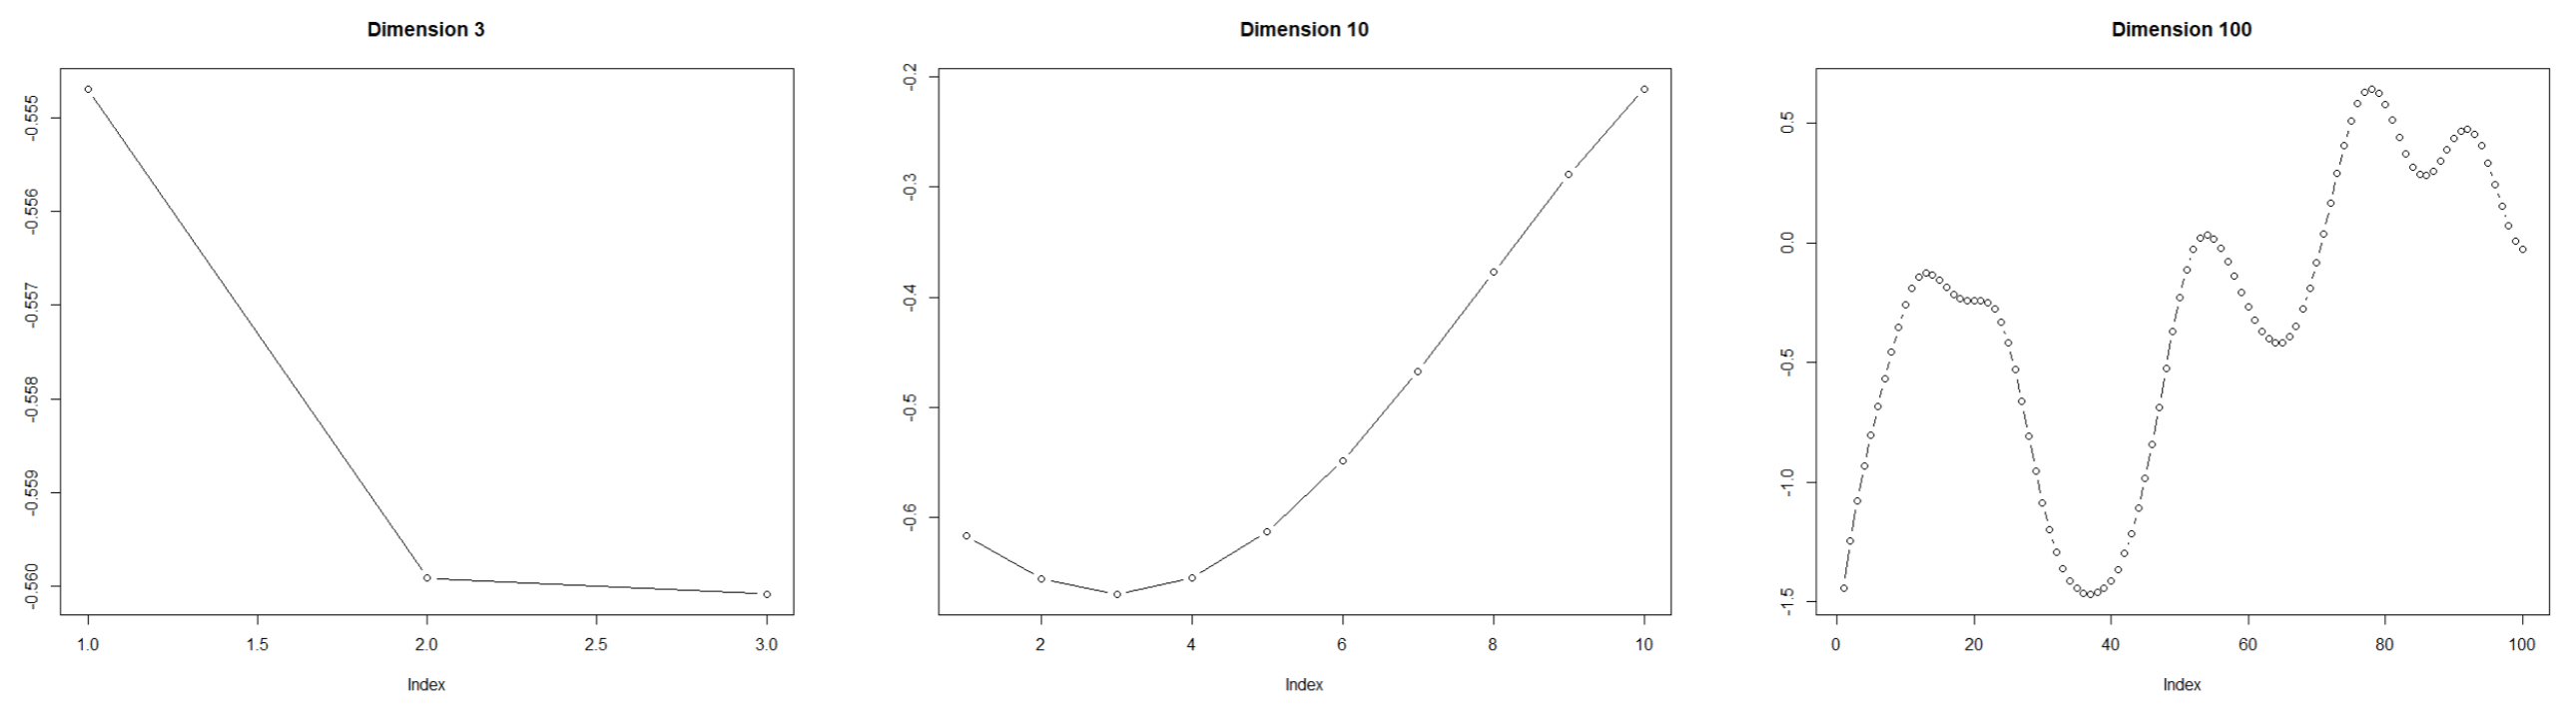
\includegraphics[width=15cm]{ex_gausses.png}
    \end{center}
    We might then consider an infinite-dimensional multivariate gaussian, and use this to approximate a function on a continuous interval, where each dimension corresponded to some $f(x_i)$, i.e. the value of the function at some given $x_i$.\\
    Formally, we write a \textit{Gaussian process} as:
    \begin{equation*}
        y(\cdot) \sim \text{GP}(\mu(\cdot),k(\cdot,\cdot))
    \end{equation*}
    $\mu(\cdot)$ is the mean function, which we will usually take to be zero, and which gives $\mathbb E[y(x)] = \mu(x)$. $k(\cdot,\cdot)$ is a \textit{covariance function}, defined so that $\cov(y(x),y(x')) = k(x,x')$. Any finite-dimensional segment of a full Gaussian process will be a multivariate distribution.\\
    There are some restrictions on the form of the covariance function, it must be:
    \begin{itemize}
        \item \textbf{Symmetric}, so that $k(x,y) = k(y,x)$ for any $x,y$.
        \item \textbf{Positive semi-definite}, so that the matrix $K_{ij} = k(x_i,x_j)$ is positive semi-definite.
    \end{itemize}
    As we assume the mean is zero, we see that the covariance function will characterise the GP to a great extent.
    % --------
    \minisection{Covariance Functions}
    A typical choice for the covariance function is a \textit{squared-exponential} (\textit{RBF}) kernel. This has a typical form:
    \begin{equation*}
        k_{\text{SE}}(x,x') = \sigma_f^2\exp\left(-\frac{\left| x--x'\right|^2}{2\ell ^2}\right)
    \end{equation*}
    Here, $\sigma_f^2$ is an associated kernel variance, and $\ell$ is a characteristic \textit{lengthscale}. For most purposes, this is the kernel we will use, though there are other choices (see relevant materials).
    % --------
    \minisection{Gaussian Process Regression}
    Consider a set of noisy observations, $y$, with known covariates $x$. Specifically, let us work with the case where this noise, $\varepsilon$, is gaussian, with a variance $\sigma_n^2$, such that $\varepsilon\sim N(0,\sigma_n^2)$. Then, for any two \textit{observed} points, their covariance is given as:
    \begin{equation*}
        \cov(y_i,y_j) = k(x_i,x_j) + \sigma_n^2\delta_{ij}
    \end{equation*}
    In the general case, we can write that:
    \begin{equation*}
        \cov(y) = K(x,x)  + \sigma_n^2\idop
    \end{equation*}
    To clarify notation, $K(x,x)$ is a matrix containing the covariance of every point with every other point, so that $K(x_i,x_j) = \cov(y_i,y_j)$ - this is a function of $x$ as the kernel (necessarily) has no dependence on $y$.\\
    Now, the goal of the regression is to find some set of points, $f'$, which approximate the underlying function over \textit{every} point $x'$. We can show that the joint distribution of $y$ and $f'$ is given:
    \begin{equation*}
        \begin{bmatrix}
            y\\ f'
        \end{bmatrix}\sim\left(
            0,\begin{bmatrix}
                K(x,x) + \sigma_n^2\idop & K(x,x')\\
                K(x',x) & K(x',x')
            \end{bmatrix}
        \right)
    \end{equation*}
    Finally, we can show that this leads to the following conditional distribution for $f'$, i.e. our prediction:
    \begin{equation*}
        f'\ |\ x,x',y \sim N(\bar f',\cov(f'))
    \end{equation*}
    Here, we have defined the mean vector, $\bar f'$, and covariance matrix, $\cov(f')$, from known quantities, as:
    \begin{align*}
        &\tcboxmath{\bar f' \equiv K(x',x)\left[ K(x,x) + \sigma_n^2\idop\right]^{-1}y}\\
        &\tcboxmath{\cov(f') \equiv K(x',x') - K(x',x)\left[ K(x,x) + \sigma_n^2\idop\right]^{-1} K(x,x')}
    \end{align*}
    We can estimate a fitted function using some measure of the point distributions, e.g. the mean fit would be constructed from the mean vector. Furthermore, we can estimate the uncertainty on this fit from the covariance matrix - specifically, the diagonal elements give the variance ($\sigma_i^2$) of each fitted point.\\
    An implementation of this regression algorithm, using numpy and scipy, can be found in my main programming file, \verb|GPs.py|.
    % --------
    \minisection{Hyperparameters}
    The main reference for this section will be section $5.4.1$ of Rasmussen and Williams, Gaussian Processes.\\
    For testing the principles of GP regression, we have the luxury of supplying our models with the exact (i.e. known) specifications of the kernel parameters, and noise variance. As such, we can achieve `pretty good' fits straight out of the box; e.g. the following, where we fit random samples taken from a RBF GP, with $\sigma^2_f=1$, $\ell=0.5$, with noise $\sigma_n^2$, using a GP with the same specifications:
    \begin{center}
        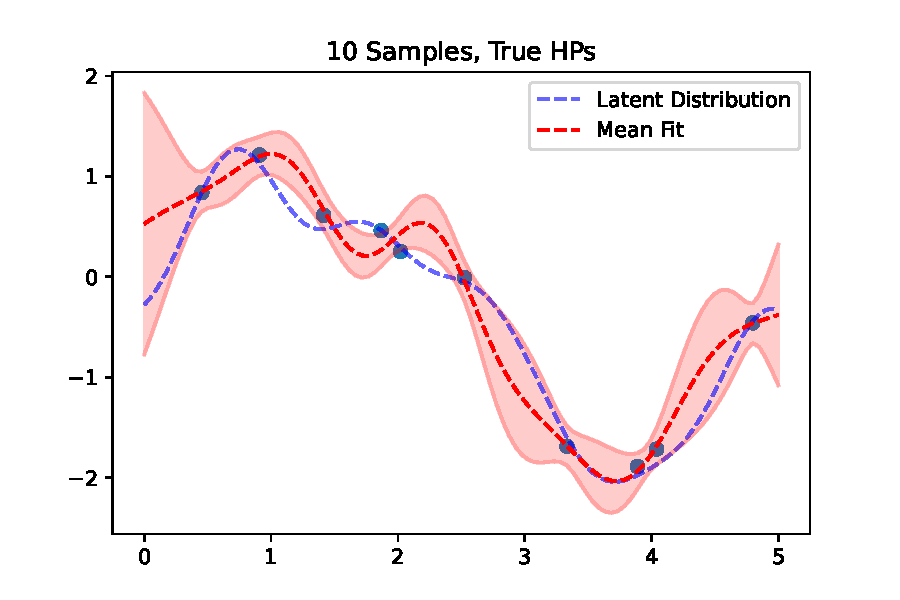
\includegraphics{hp_known.pdf}
    \end{center}
    In practice, though, we will not actually know these `exact' specifications (if they exist at all), and will need to estimate a set of hyperparameters for the dataset. One quantity which proves particularly useful in this regard is the \textit{marginal likelihood} of observing the data $p(y\ |\ x)$, given a particular model specification. The log-form is simplest to work with (defining $K_{xx}\equiv K(x,x)$):
    \begin{equation*}
        \log p(y\ |\ x) = -\frac 12 y^T\left[ K_{xx} + \sigma_n^2\idop\right]^{-1}y - \frac 12\log\left| K_{xx} + \sigma_n^2\idop\right| - \frac n2\log 2\pi
    \end{equation*}
    The final term has no dependence on the HPs, so we are only really interested in the first two. Maximising this log-likelihood (or, equivalently, minimising the negative log-likelihood) with respect to the hyperparameters will then yield an estimate.\\
    For the same case as above, if we take $\sigma_f^2=1$, then we can minimise the negative log-likelihood with respect to $\ell$ and $\sigma_n^2$ to find estimates for these hyperparameters:
    \begin{center}
        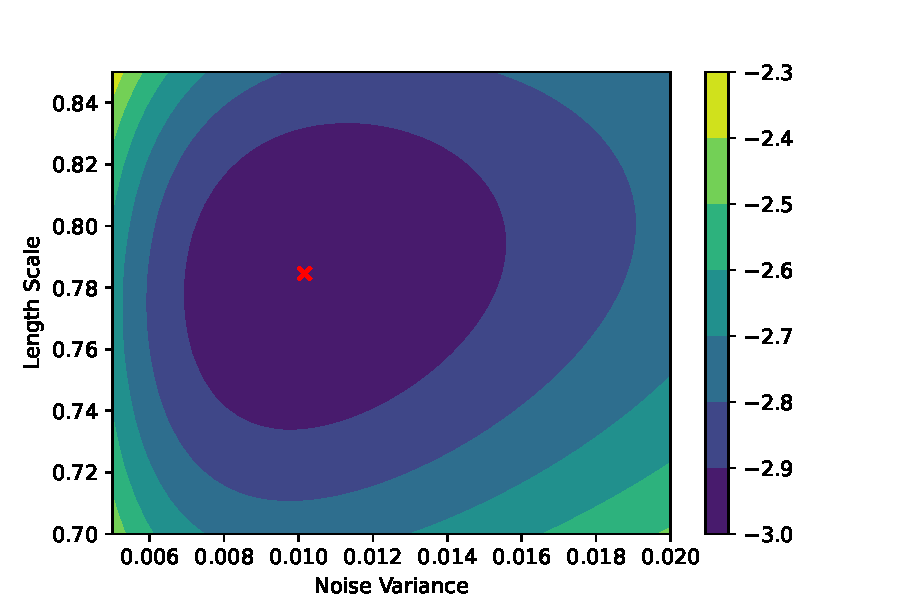
\includegraphics{hp_contours.pdf}
    \end{center}
    This can be achieved numerically (as it is above). In this specific example (seed $140725984$), we find MLE estimates $\ell \simeq 0.785$ and $\sigma_n^2 \simeq 0.0102$, which are quite close to the `actual' values. Regression under these specification yields a fairly good fit, in fact:
    \begin{center}
        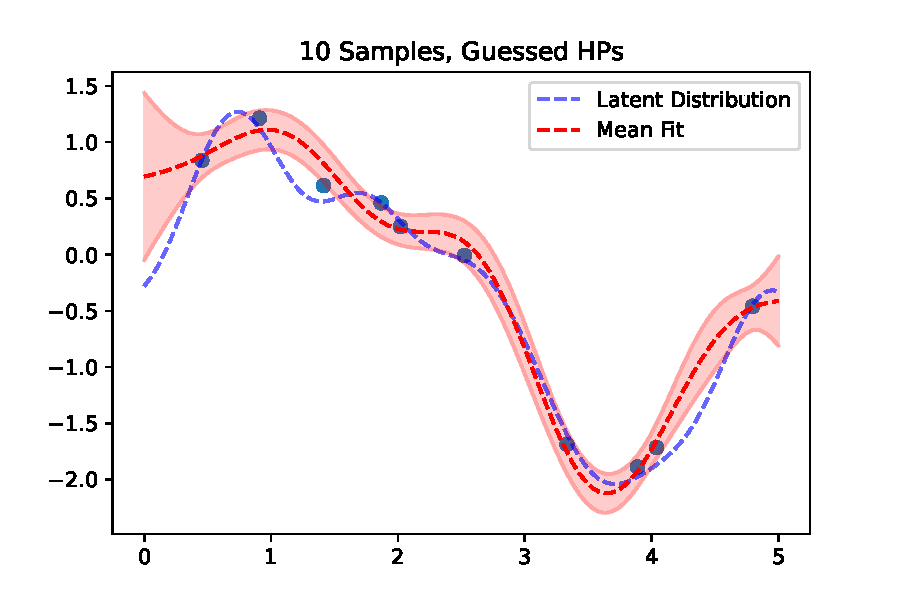
\includegraphics{hp_fitted.pdf}
    \end{center}
    This being said, the effectiveness of this method varies - the log-likelihood may have local maxima, and the noise variance (particularly) is prone to being largely underestimated or overestimated.\\
    A log-likelihood minimisation routine is implemented in the \verb|GPs.py| program (though the plotting is quite inefficient).

    \newpage
    % Questions!
    \doubleline
    \begin{center}
        \huge \textbf{Questions}
    \end{center}
    \doubleline
    \begin{center}
        \hrule\vspace*{0.25cm}
        \textbf{I} - \textit{For the covariance function, or kernel, k of a GP, what information does it represent about any two points in the domain?}\vspace*{0.25cm}\hrule
    \end{center}
    The covariance function, $k$, of a GP dictates the covariance between any two given points, so that:
    \begin{equation*}
        \cov\big(f(x_1),f(x_2)\big) = k(x_1,x_2) = k(x_2,x_1)
    \end{equation*}
    That is to say, a large positive covariance between two random variables means that, if one is measured to be large (as compared to the mean), then the other will also likely be large, and vice versa.\\
    In the context of a GP, this essentially specifies the form of the function generated.
    \begin{center}
        \hrule\vspace*{0.25cm}
        \textbf{II} - \textit{Assume that you know the exact GP model specification. Given some observation with additive Gaussian noise, how would you use those to predict the expected value (and uncertainty) of an unobserved location?}\vspace*{0.25cm}\hrule
    \end{center}
    \dots
    \begin{center}
        \hrule\vspace*{0.25cm}
        \textbf{III} - \textit{Draw samples from a GP with one-dimensional input, zero-mean, RBF kernel with variance 1 and lengthscale 0.5.}\vspace*{0.25cm}\hrule
    \end{center}
    An RBF kernel with variance $1$, and lengthscale $0.5$, is mathematically given as:
    \begin{equation*}
        k_{RBF}(x,x') = \exp\left(\frac{\left| x-x'\right|^2}{2}\right)
    \end{equation*}
    Using numpy and scipy (for multivariate sampling), I have plotted three samples from this GP, with $x\in (0,5)$ and $N=100$:
    \begin{center}
        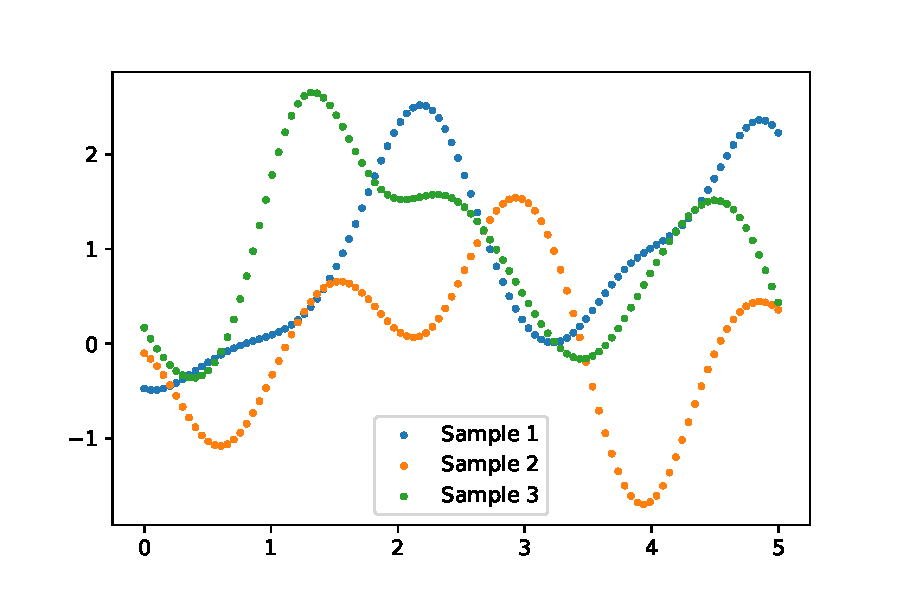
\includegraphics{sampling.pdf}
    \end{center}
    \begin{center}
        \hrule\vspace*{0.25cm}
        \textbf{IV} - \textit{Do GP regression with observations made using an arbitrary sample from the above GP model (with additive, i.i.d. Gaussian noise of variance $0.01$)}\vspace*{0.25cm}\hrule
    \end{center}
    This has been demonstrated in the previous section. See \verb|GPs.py| for the implementation.
    \begin{center}
        \hrule\vspace*{0.25cm}
        \textbf{V} - \textit{How would the computational cost of predicting the distribution of the GP at a new location scale as the number of observations increases? Show mathematically and support it with evidence from numerical experiments.}\vspace*{0.25cm}\hrule
    \end{center}
    The main cost in prediction will come from inversion of the $n\times n$ matrix, where $n$ is the number of observations:
    \begin{equation*}
        \bar f'_i = K(x'_i,x) \cdot \left[ K(x,x) + \sigma_n^2\idop\right]^{-1}\cdot y
    \end{equation*}
    $K(x'_i,x)$ and $y$ will be row and column vectors of length $n$, respectively.\\
    In the documentation for \verb|np.linalg.inv()|, it states a time complexity $O(n^3)$. However, numerical observations seem to indicate a linear scaling:
    \begin{center}
        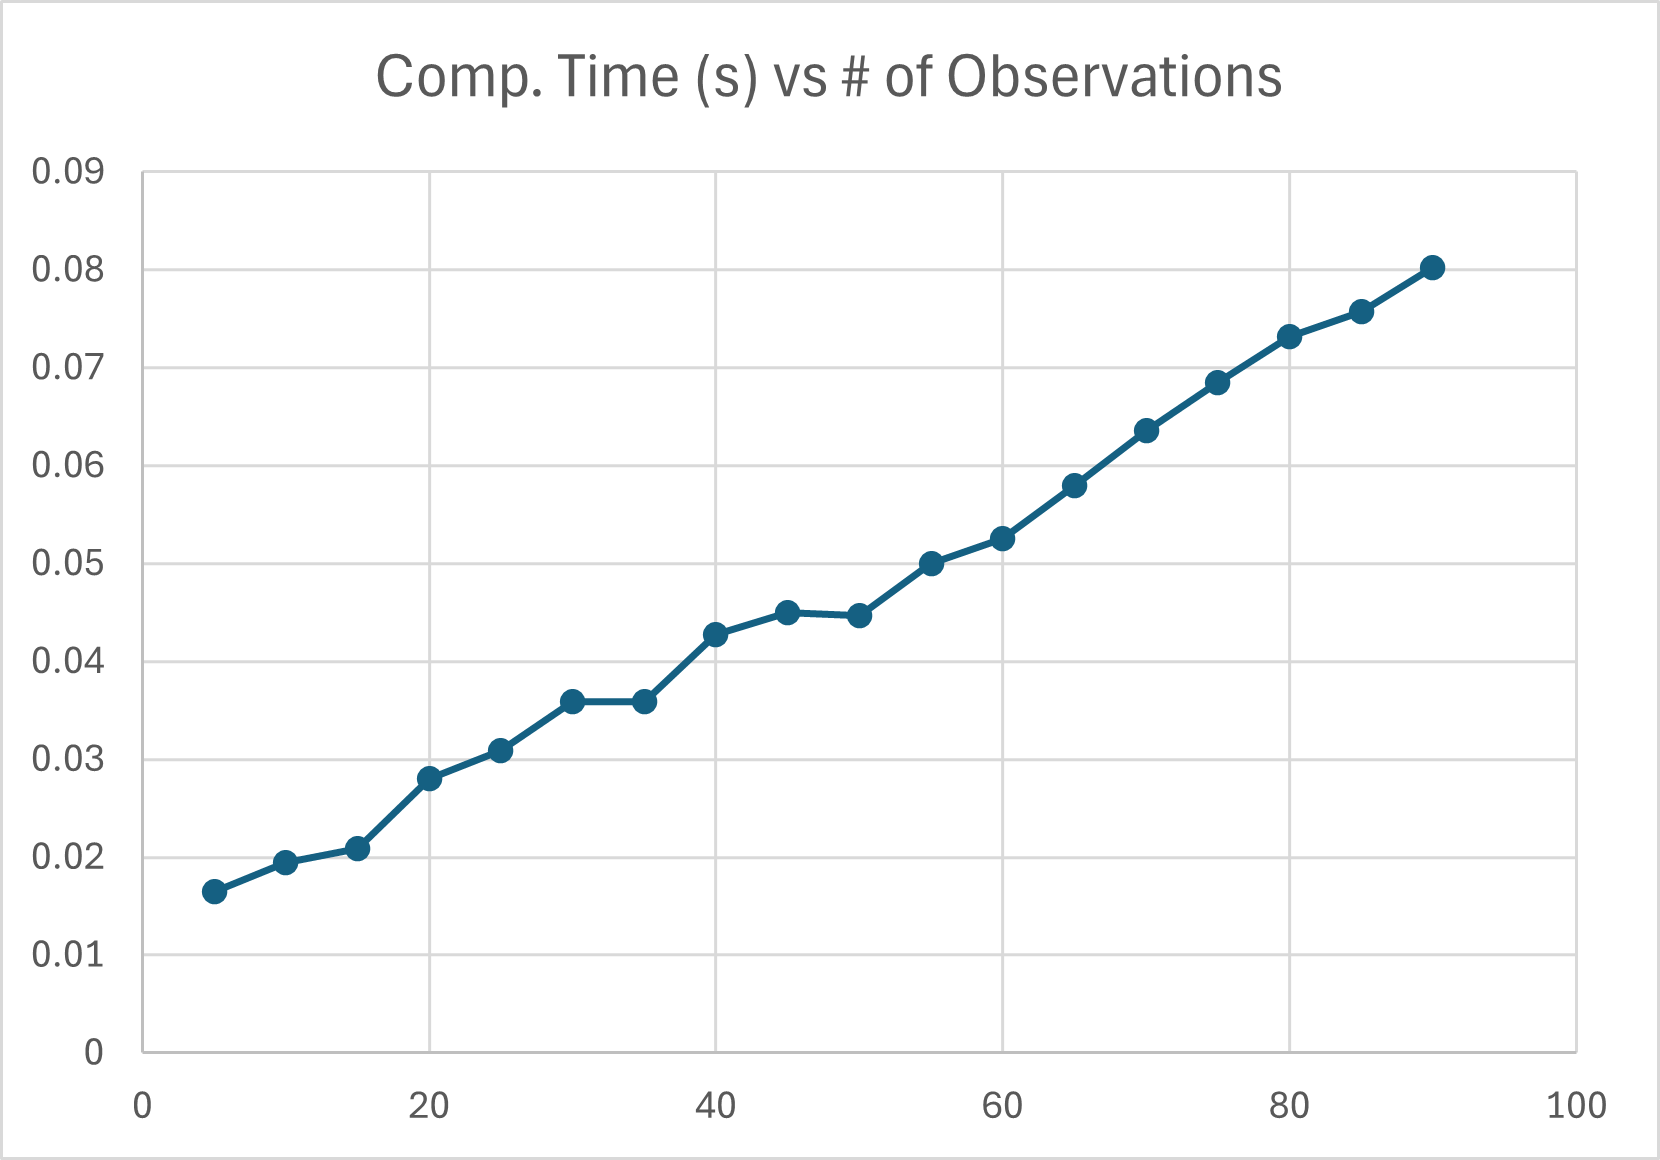
\includegraphics{timescaling.png}
    \end{center}
\end{document}